\documentclass[10pt]{article}

%Math
\usepackage{amsmath}
\usepackage{amsfonts}
\usepackage{amssymb}
\usepackage{amsthm}
\usepackage{ulem}
\usepackage{stmaryrd} %f\UTF{00FC}r Blitz!

%PageStyle
\usepackage[ngerman]{babel} % deutsche Silbentrennung
\usepackage[utf8]{inputenc} 
\usepackage{fancyhdr, graphicx}
\usepackage[scaled=0.92]{helvet}
\usepackage{enumitem}
\usepackage{parskip}
\usepackage[a4paper,top=2cm]{geometry}
\setlength{\textwidth}{17cm}
\setlength{\oddsidemargin}{-0.5cm}


% Shortcommands
\newcommand{\Bold}[1]{\textbf{#1}} %Boldface
\newcommand{\Kursiv}[1]{\textit{#1}} %Italic
\newcommand{\T}[1]{\text{#1}} %Textmode
\newcommand{\Nicht}[1]{\T{\sout{$ #1 $}}} %Streicht Shit durch

%Arrows
\newcommand{\lra}{\leftrightarrow} 
\newcommand{\ra}{\rightarrow}
\newcommand{\la}{\leftarrow}
\newcommand{\lral}{\longleftrightarrow}
\newcommand{\ral}{\longrightarrow}
\newcommand{\lal}{\longleftarrow}
\newcommand{\Lra}{\Leftrightarrow}
\newcommand{\Ra}{\Rightarrow}
\newcommand{\La}{\Leftarrow}
\newcommand{\Lral}{\Longleftrightarrow}
\newcommand{\Ral}{\Longrightarrow}
\newcommand{\Lal}{\Longleftarrow}

% Code listenings
\usepackage{color}
\usepackage{xcolor}
\usepackage{listings}
\usepackage{caption}
\DeclareCaptionFont{white}{\color{white}}
\DeclareCaptionFormat{listing}{\colorbox{gray}{\parbox{\textwidth}{#1#2#3}}}
\captionsetup[lstlisting]{format=listing,labelfont=white,textfont=white}
\lstdefinestyle{JavaStyle}{
 language=Java,
 basicstyle=\footnotesize\ttfamily, % Standardschrift
 numbers=left,               % Ort der Zeilennummern
 numberstyle=\tiny,          % Stil der Zeilennummern
 stepnumber=5,              % Abstand zwischen den Zeilennummern
 numbersep=5pt,              % Abstand der Nummern zum Text
 tabsize=2,                  % Groesse von Tabs
 extendedchars=true,         %
 breaklines=true,            % Zeilen werden Umgebrochen
 frame=b,         
 %commentstyle=\itshape\color{LightLime}, Was isch das? O_o
 %keywordstyle=\bfseries\color{DarkPurple}, und das O_o
 basicstyle=\footnotesize\ttfamily,
 stringstyle=\color[RGB]{42,0,255}\ttfamily, % Farbe der String
 keywordstyle=\color[RGB]{127,0,85}\ttfamily, % Farbe der Keywords
 commentstyle=\color[RGB]{63,127,95}\ttfamily, % Farbe des Kommentars
 showspaces=false,           % Leerzeichen anzeigen ?
 showtabs=false,             % Tabs anzeigen ?
 xleftmargin=17pt,
 framexleftmargin=17pt,
 framexrightmargin=5pt,
 framexbottommargin=4pt,
 showstringspaces=false      % Leerzeichen in Strings anzeigen ?        
}

%Config
\renewcommand{\headrulewidth}{0pt}
\setlength{\headheight}{15.2pt}

%Metadata
\fancyfoot[C]{If you use this documentation for a exam, you should offer a beer to the authors!}
\title{
	\vspace{5cm}
	Systemprogrammierung \\
	Test 2
}
\author{Jan Fässler}
\date{3. Semester (HS 2012)}


% hier beginnt das Dokument
\begin{document}

% Titelbild
\maketitle
\thispagestyle{fancy}

\newpage

% Inhaltsverzeichnis
\pagenumbering{Roman}
\tableofcontents	  	


\newpage
\setcounter{page}{1}
\pagenumbering{arabic}

% Inhalt Start

\section{Sockets}
Die Socket Schnittstelle wurde an der University of California entwickelt. Ziel war es eine offene, generische Programmierschnittstelle für die Interprozesskommunikation für UNIX zu realisieren. Sockens erlauben es dem Nutzer sich mit dem Netzwerk zu verbinden. Der Socket ist dabei der Endpunkt einer Kommunikationsverbindung, wie zum Beispiel eine Telefonsteckdose. Die Anforderungen an die Schnittstelle waren:
\begin{description}
	\item[Transparenz] bezüglich Netzwerkverhalten
	\item[Effizienz] um die Programmierer zu überzeugen
	\item[Kompatibilität] mit dem UNIX Standard I/O
\end{description}

\subsection{Grundkonzepte}
\begin{description}
	\item[communication domains] \hfill \\ Unterstützung verschiedener Netzwerkprotokolle
	\item[communication types] \hfill \\ Klassifikation von Eigenschaften
	\item[name binding] \hfill \\ Bennenung und Adressierung von Endpunkten
	\item[Sockets] \hfill \\ Einheiltiche Abstraktion von Endpunkten
\end{description}

\subsection{Erstellen einer Socket Verbindung}
\begin{center}
	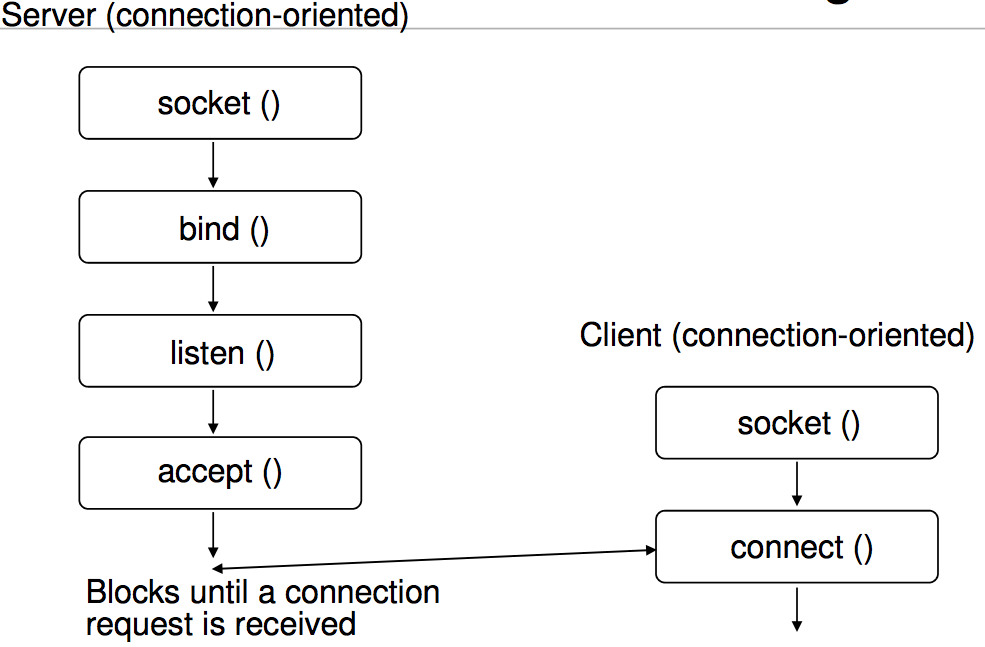
\includegraphics[scale=0.2]{socket-verbindungsaufbau.png}
\end{center}

\subsection{Senden und Empfangen von Daten}
Um möglichst viele Domänen (Unix, Internet, ...) und Protokolle (TCP, UDP, ...) zu unterstützen, gibt es verschiedene Paare von System Calls welche aber in den meisten UNIX Varianten auf einer einzigen internen Funktion abgebildet werden.
\begin{description}
	\item[read/write] \hfill \\ Rückwärtskompatibilität zum UNIX Standard I/O, ermöglichen von Pipes mit dup()
	\item[send/recv] \hfill \\ zusätzliche Funktionalität und Parametrisierung  nutzt TCP, Packete geordnet
	\item[sendto/recvfrom] \hfill \\ erlaubt senden ganzer Datagramme ohne Verbindung (UDP), Packete ungeordnet, keine Fehlerüberprüfung, zwei Buffer nötig (Sender/Empfänger)
	\item[sendmsg/recvmsg] \hfill \\ nicht Bytestrom orientiert, Appl. wird erst benachrichtig wenn die ganze Nachricht angekommen ist.
\end{description}

\subsection{Blockierendes vs. selektives Warten auf Sockets}
\begin{description}
	\item[accept()] \hfill \\ Blockiert den aufrufenden PRozess solange, bis ein Verbindungsaufbauwunsch am Socket signalisiert wird
	\item[select()] \hfill \\ Erlaubt nicht blockierendes Warten auf eine Verbindung
\end{description}

\subsection{Beenden einer Verbindung}
\begin{description}
	\item[shutdown()] \hfill \\ Signalisiert Verbinungsabbruch der anderen Seite und wartet auf eine Bestätigung. Vor der Bestätigung eintreffende Daten werden noch bestätigt, jedoch nicht an die Appl. weitergegeben. Ein beenden kann einseitig oder beidseitig erfolgen.
	\item[close()] \hfill \\ Dealloziert die lokale Socket Datenstruktur und die zugerdneten Ressourcen (Puffer)
	\item[exit()] \hfill \\ Terminiert das PRogramm ohne explizites shutdown/close. Es überlässt die Aufräumarbeiten dem OS und der Gegenpartei.
	\item[Provider Abort] \hfill \\ überlässt das Afuräumen dem OS beider Gegenparteien
\end{description}

\subsection{Speicherverwaltung auf der Socket Schicht}
Daten auf einem socket werden in sogenannten mbufs gespeichert, welche jeweils auf den folgenden mbuf verweisen (wie eine LinkedList). Alle mbufs zusammen sind der mbuf Pool.
\begin{center}
	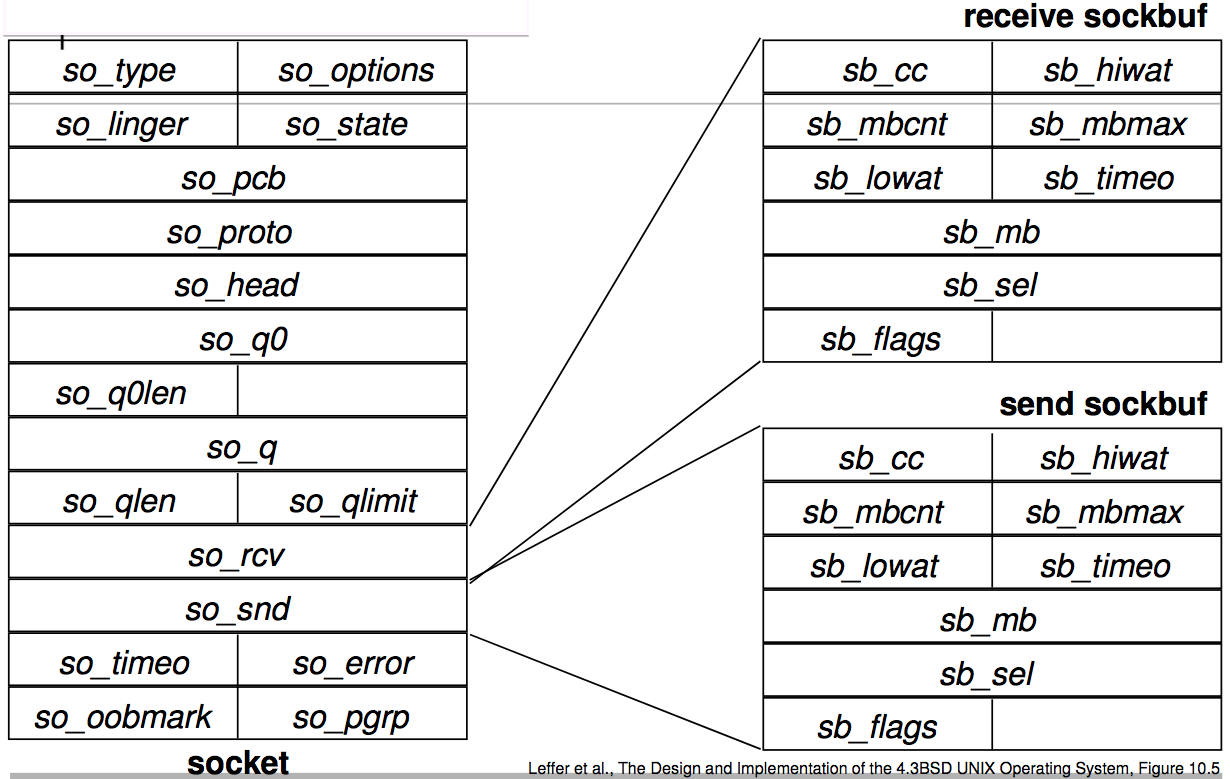
\includegraphics[scale=0.2]{socket-datenstruktur.png}
\end{center}
\begin{center}
	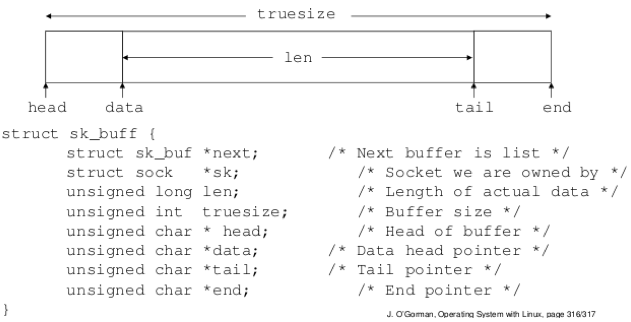
\includegraphics[scale=0.5]{socket-buffer.png}
\end{center}

\subsection{Datenfluss duch die Schichten}
\begin{center}
	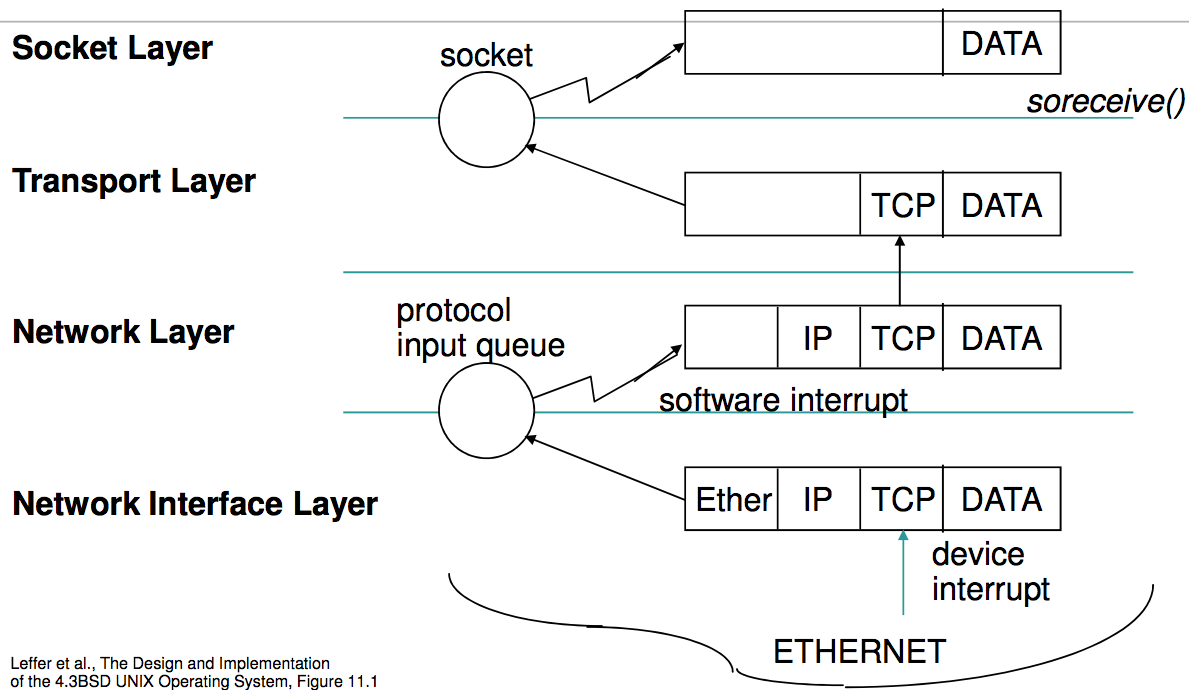
\includegraphics[scale=0.2]{socket-datenfluss.png}
\end{center}

\subsection{System Calls}
\begin{description}
	\item[socket(domain, type, prot)] \hfill \\ Socket erstellen
	\item[bind(sockfd, addr, addlen)] \hfill	\\ Nach dem Erstellen eines Sockets existiert dieser blos als Name aber er hat noch keine Adresse. Bind verknüpft ihn mit einer Adresse.
	\item[listen(sockfd, backlog)] \hfill \\ Markiert den Socket als passiven Socket. Das bedeutet als Socket der einkommende Verbindungen mit accept entgegennehmen kann.
	\item[accept(socketfd, addr, addlen, flags)] \hfill \\ Wird mit Verbindungsbassierten Socket Typen (STREAM, SEQPACKET) verwendet. Entpackt die erste Anfrage au der Queue der zu berarbeitenden Verbindungen für den hörenden Socket. Kreiert einen neuen verbundenen Socket und gibt einen neuen File Descriptor zurück, welcher auf diesen verweist. Der ursprüngliche Socket wird nicht verändert. Der neue ist nicht im listening state.
	\item[connect(socketfd,addr,addrlen)] \hfill \\ Verbindet den Socket zur Adresse.
\end{description}


\newpage
\section{Interprocess Communication (IPC)}
\subsection{Zentrale Konzepte}
Es gibt im System drei verschiedene IPC MEchanismen, für deren Verwaltung der Kernel je eine separate Tabelle pflegt: \textbf{Message Queues}, \textbf{Shared Memory} und \textbf{Semaphore}. \\
Für die Verwaltung  aller drei Mechanismen werden \textbf{dieselben Prozeduren} verwendet. Der Zugriff erfolgt über \textbf{einen numerischen Schlüssel}. Es gibt keine Registratur für verwendete/reservierte Schlüssel. \textbf{Kollisionen sind also möglic}h. Die IPC Objekte sind \textbf{nicht kompatibel mit dem Standard I/O} bassierter Prozesskommunikation wie Dateinen, Sockets, Pipes oder Geräte. Sie sind alle \textbf{limitiert auf ein lokales System}.

\subsection{Verwaltung der Objekte}
\begin{center}
	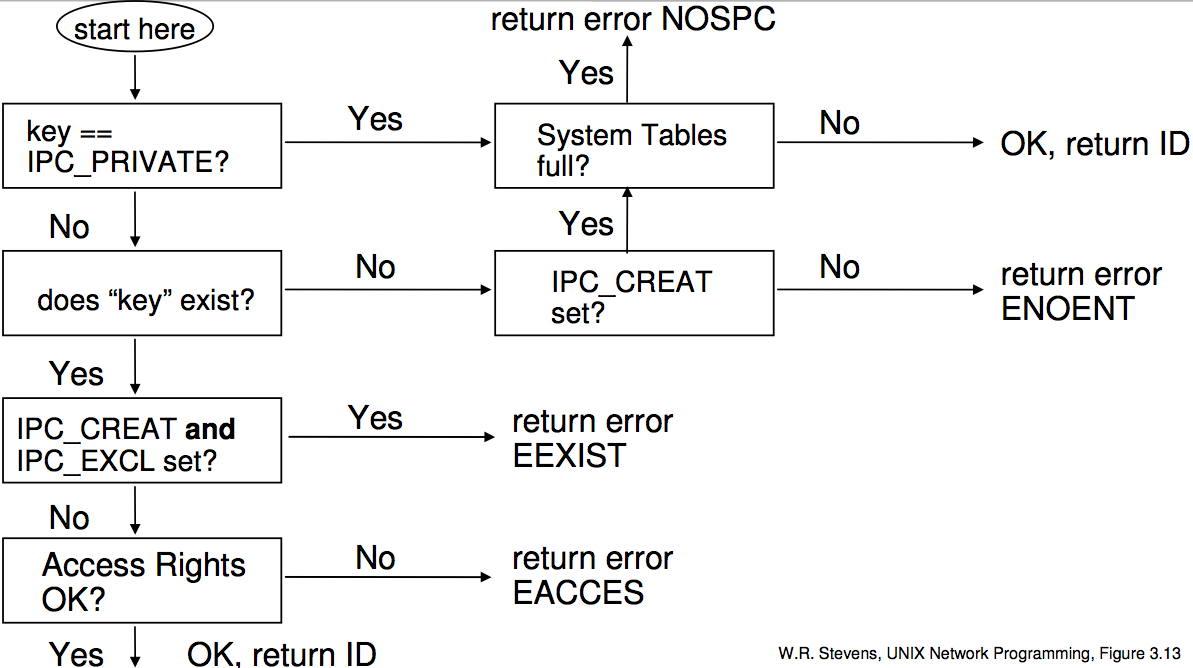
\includegraphics[scale=0.2]{ipc-verwaltung.png}
\end{center}

\newpage
\subsection{Shared Memory}
Shared Memory erlaubt die gemeinsame Nutzung von Hauptspeicher-Seiten zwischen verschidenen (nicht) verwandten Prozessen. Es wird ein dedizierter Segment Typ verwendet, der auf der normalen Speicherverwaltung basiert. Die Synchronisation muss über Semaphore, Signalbits oder allgemeine Signale erfolgen.
\begin{center}
	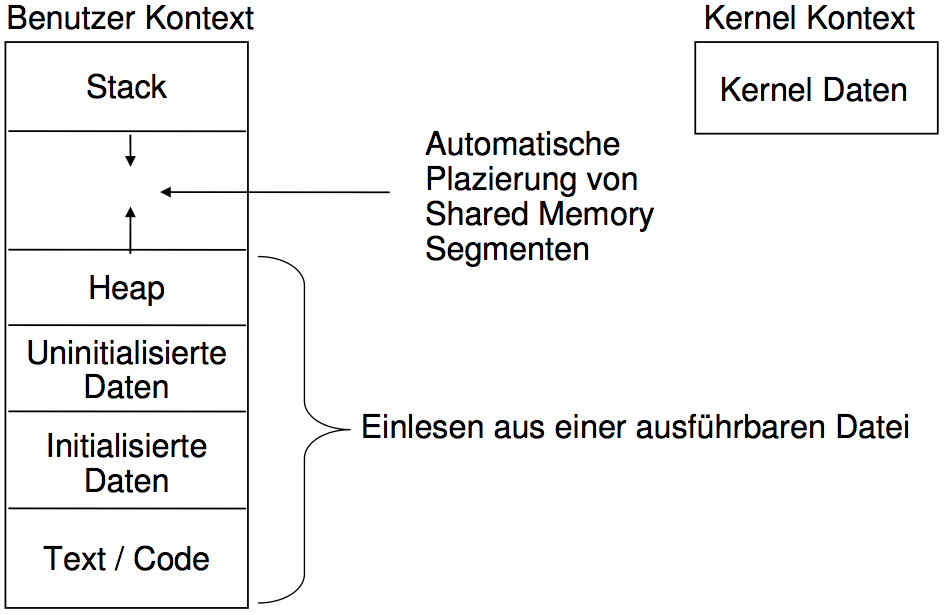
\includegraphics[scale=0.2]{sharedmemory-process-adress.png}
\end{center}

\subsubsection{Erstellen eines Segmentes (shmget)}
\begin{itemize}
	\item Entfernen einer Region von der Liste freier Regionen
	\item Einen Typ zuweisen
	\item Einen inode Pointer zuweisen
	\item Den reference count der inode um eins erhöhen
	\item region der Liste von aktiven Regionen hinzufügen
	\item gesperrete Region zurückgeben.
\end{itemize}
\begin{lstlisting}[language=Java, caption=Erstellen eines Shared Memory Segments, style=JavaStyle]
int size, permflags, shm_id; key_t key;
shm_id = shmget (key, size, permflags);
\end{lstlisting}

\subsubsection{Einbinen eines Segmentes (shmat)}
\begin{itemize}
	\item check validity of descriptor, permissions 
	\item if (user specified virtual address)
		\begin{itemize}
			\item round off virtual address, as specified by flags;
			\item check legality of virtual address, size of region;
		\end{itemize}
	\item else - kernel picks virtual address: error if none available;
	\item attach region to process address space (algorithm attachreg);
	\item if (region being attached for the first time)
		\begin{itemize}
			\item allocate page tables, memory for region (algorithm growreg);
		\end{itemize}
	\item return (virtual address where attached);
\end{itemize}
\begin{lstlisting}[language=Java, caption=Einbindung eines Shared Memory Segments, style=JavaStyle]
int shm_id, shmflags; char *memptr, *daddr, *shmat();
memptr = shmat (shm_id, daddr, shmflags);
\end{lstlisting}

\subsubsection{Entfernen eines Segmentes (shmdt)}
\begin{itemize}
	\item get auxiliary memory management tables for process,
	\item release as appropriate;
	\item decrement process size;
	\item decrement region reference count;
	\item if (region count is 0 and region not sticky bit)
		\begin{itemize}
			\item free region (algorithm freereg);
		\end{itemize}
	\item else \textit{/* either reference count non-0 or region sticky bit on */}
		\begin{itemize}
			\item free inode lock, if applicable (inode associated with region);
			\item free region lock;
		\end{itemize}
\end{itemize}
\begin{lstlisting}[language=Java, caption=Entfernen eines Shared Memory Segments, style=JavaStyle]
int       retval; char      *memptr;
retval = shmdt (memptr);
\end{lstlisting}

\subsubsection{System Calls}
\begin{description}
	\item[shmget(key, size, shmflag)] \hfill \\ Gibt ID des Shared Memory Segments entsprechenden
	\item[shmat(shmid, shmaddr, shmflg)] \hfill \\ Attach: Fügt das  Segment zum Addressspace des Prozesses hinzu.
	\item[shmdt(shmaddr)] \hfill \\ Detach: Entfernt das Segemnt vom Addressspace des Prozesses
	\item[shmctl(shmid,cmd,*buf)] \hfill \\ Fürht cmd auf dem Segment aus
\end{description}

\newpage
\subsection{Message Queues}
Message Queues dienen zum Versenden von Datenmengen von einem Server an einen Client. Sie ist eine verkettete Liste wobei die Liste vom Listenkopf aus kontrolliert wird. Mit msgsend() werden Elemente an die Schlange angefügt und mit msgrcv() gelesen und wieder entfernt. Es können beliebige strukturierte Daten ausgetauscht werden zwischen verdandten oder nicht verwandten Prozessen.

\subsubsection{Erzeugen einer Message Queue}
Durch den Aufruf von msget() besorgt sich ein Prozess den Zugriff auf eine message queue id. Mit msgctl() kann diese gelöscht, gelesen, modifiziert, gesperrt oder entsperrt werden.
\begin{lstlisting}[language=Java, caption=Erzeugen einer Message Queue, style=JavaStyle]
int msg_qid, permflags; key_t key;
msg_qid = msgget (key, permflags);
\end{lstlisting}

\subsubsection{Senden einer Nachricht}
\begin{itemize}
	\item check legality of descriptor, permissions;
	\item while (not enough space to store message) 
		\begin{itemize}
			\item if (flags specify not to wait) return;
			\item sleep (until event enough space is available);
		\end{itemize}
	\item get message header;
	\item read message text from user space to kernel;
	\item adjust data structures:
		\begin{itemize}
			\item enqueue message header,
			\item message header points to data,
			\item counts,
			\item time stamps,
			\item process ID;
		\end{itemize}
	\item wakeup all processes waiting to read message from queue;
\end{itemize}
\begin{lstlisting}[language=Java, caption=Versenden einer Nachricht, style=JavaStyle]
int msg_qid, size, flags, retval;
struct my_msg {
	long mtype;
	char mtext[SOMEVALUE];
} message;
retval = msgsnd (msg_qid, &message, size, flags);
\end{lstlisting}

\subsubsection{Empfang einer Nachricht}
\begin{itemize}
	\item check permissions;
	\item \textbf{loop;}
	\item check legality of message descriptor;
	\item \textit{/* find message to return to user */}
	\item \textbf{if (requested message type $==$ 0)}
		\begin{itemize}
			\item consider first message on queue;
		\end{itemize}
	\item \textbf{else if (requested message type $>$ 0)}
		\begin{itemize}
			\item consider first message on queue with given type;
		\end{itemize}
	\item else   \textbf{/* requested message type $<$ 0 */}
		\begin{itemize}
			\item consider first of the lowest typed messages on queue, such that its type is $<=$ absolute value of requested type;
		\end{itemize}
	\item if (there is a message )
		\begin{itemize}
			\item adjust message size or return error if user size too small;
			\item copy message type, text from kernel space to user space;
			\item unlink message from queue;
			\item return;
		\end{itemize}
	\item \textit{/* no message */}
	\item if (flags specify not to sleep) return with error;
	\item sleep (event message arrives on queue);
	\item \textbf{goto loop;}
\end{itemize}
\begin{lstlisting}[language=Java, caption=Empfangen einer Nachricht, style=JavaStyle]
int msg_qid, size, flags, retval; long msg_type;
struct my_msg { 
	long mtype;
	char mtext[SOMEVALUE];
} message;

retval = msgrcv (msg_qid, &message, size, msg_type, flags);
\end{lstlisting}

\newpage
\subsection{Semaphore}
Ein Semaphor ist zwar kein Mechanismus für die Datenübertragung, erkann jedoch hilfreich sein für die Synchronisierung der Prozesse.Vereinfacht gesprochen ist ein Semaphor ein Zähler, dessen Wert entscheidet, ob eine Ressource eklusiv nutzbar ist oder nicht. Er besteht aus einem Zähler und einer Warteschlange für die Aufnahme blockierter Prozesse. Er hat drei Funktionen:
\begin{description}
	\item[initsem()] \hfill \\ Initialisierungsfunktion
	\item[P()] \hfill \\ Prüfen und dekrementieren des Semaphor. Falls er danach noch grösser als null ist, setzt der Prozess seine Arbeit fort, ansonsten wartet er.
	\item[V()] \hfill \\ Der Semaphor erhöhen, was eventuell wartende Prozesse wieder freigibt.
\end{description}

\subsubsection{Benutzung für gegenseitigen Ausschluss}
In einem kritischen Abschnitt verändert Prozess P1 eine Datenstruktur, die der Prozess gemeinsam mit einem Prozess P2 nutzt. Prozess P2 verändert die Datenstruktur in seinem kritischen Abschnitt. Ein Semaphor in Ausschlussfunktion wird eingesetzt, um zu erreichen, dass sich die Prozesse P1 und P2 niemals gleichzeitig in ihren kritischen Abschnitten befinden. Hierzu wird der Semaphor mit 1 initialisiert
\begin{center}
	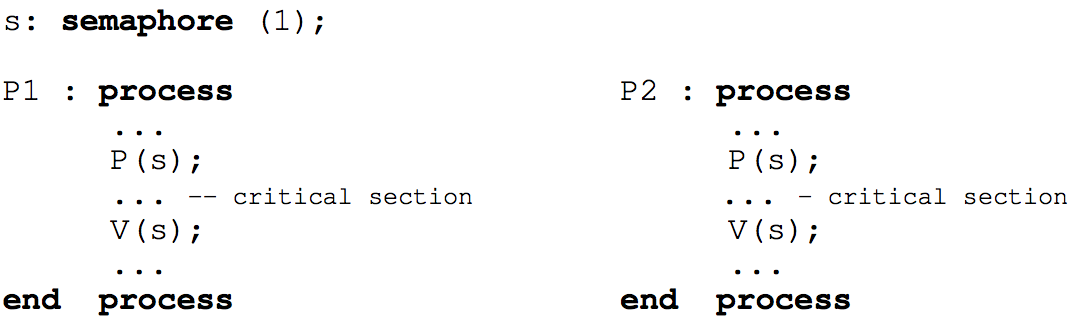
\includegraphics[scale=0.25]{semaphore-benutzung-ausschluss.png}\\
\end{center}

\subsubsection{Benutzung für Prozess-Synchronisation}
Der Prozess P1 beginnt mit einem kritischen Abschnit gleich nach der Initialisierung. Der Prozess P2 kann vorerst nur bis zu der P-Funktion laufen, da der Semaphor mit 0 initialisiert wurde. Erst wenn P1 mit der V-Funktion den Zähler um eins incrementiert kann der Prozess P2 weiterlaufen.
\begin{center}
	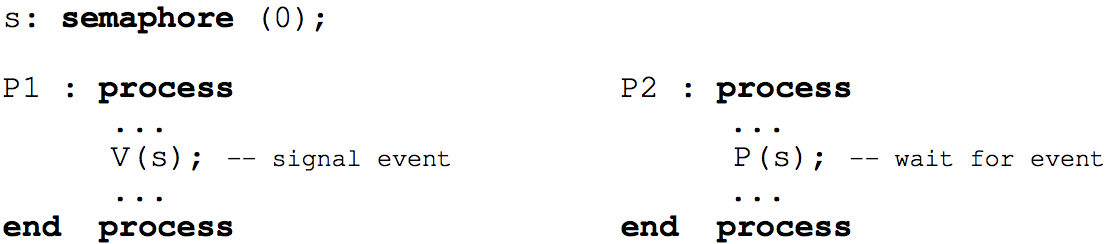
\includegraphics[scale=0.25]{semaphore-benutzung-synchronisation.png}\\
\end{center}

\subsubsection{Additive Semaphore}
\begin{center}
	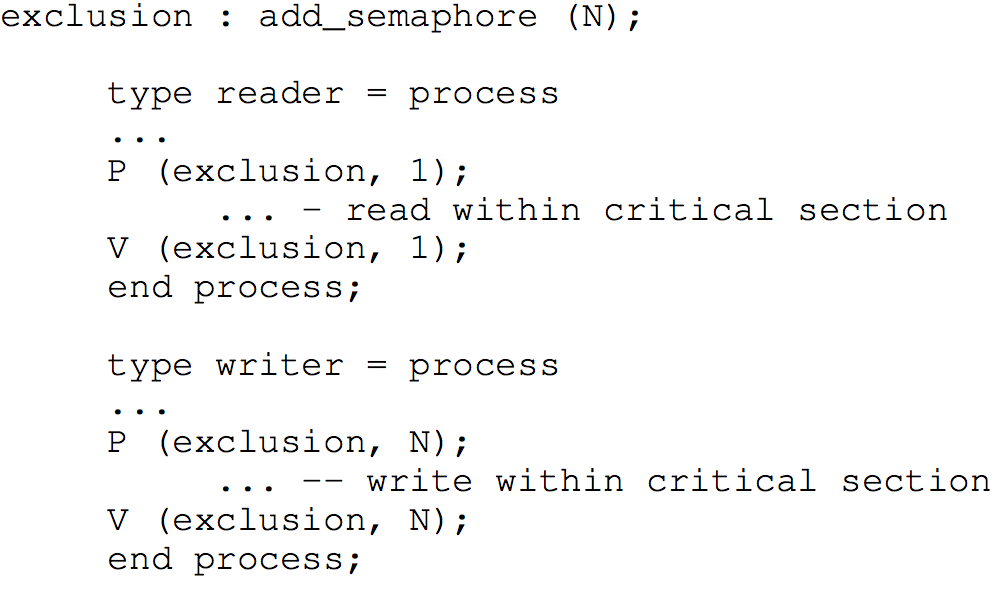
\includegraphics[scale=0.25]{semaphore-additive.png}\\
\end{center}

\subsubsection{Beispiel}
\begin{lstlisting}[language=Java, caption=Semaphore Beispiel, style=JavaStyle]
P (semid) int semid; {
     struct sembuf p_buf;
     p_buf.sem_num = 0;
     p_buf.sem_op = -1;        /* negativer Wert, also Fall 1 = P() */
     p_buf.sem_flg = SEM_UNDO;
     if (semop (semid, &p_buf, 1) == -1) {
          perror (?p(semid) failed?);
          exit (1);
     } else return (0);
}
V (semid) int semid; {
     struct sembuf v_buf;
     v_buf.sem_num = 0;
     v_buf.sem_op = 1;        /* positiver Wert, also Fall 2 = V() */
     v_buf.sem_flg = SEM_UNDO;
     if (semop (semid, &v_buf, 1) == -1) {
          perror (?v(semid) failed?);
          exit (1);
     } else return (0);
}

main () {
     key_t semkey = 0x200;
     if (fork () == 0) handlesem (semkey);
     if (fork () == 0) handlesem (semkey);
     if (fork () == 0) handlesem (semkey);
}
handlesem (skey) key_t skey; {
     int semid, pid = getpid();
     if ((semid = initsem (skey)) > 0) exit (1);
     printf (?\nprocess %d before critical section\n?, pid); 
     P (semid);
     printf (?process %d in critical section\n?, pid);
     sleep (2);
     printf (?process %d leaving critical section\n?, pid); 
     V (semid);
     printf (?process %d exiting\n?, pid);
     exit (0);
}
\end{lstlisting}

\newpage
\section{Remote Procedure Calls}
RPC ist eine Technik zur Realisierung von Interprozesskommunikation zwischen verschidenen Rechnern. Es gibt verschiedene Implementierungen welche meist nicht untereinander kompatiebel sind.
\begin{center}
	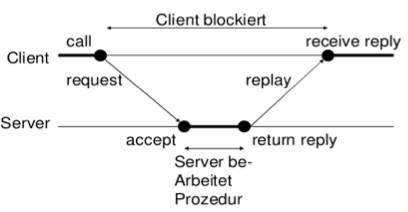
\includegraphics[scale=0.5]{rpc.png}\\
\end{center}

\subsection{Funktionsweise}
Der Client ruft eine entfernte Prozedur auf einem Server auf. Die zur Bearbeitung benötigten Parameter werden an die Client-Stub Funktionsstelle des RPC Systems geschickt. Die Stub verpackt alle Funktionsparameter in eine komplexe Datenstruktur – dieser Vorgang wird auch "Marshalling" genannt. \\
Danach beauftragt die Stub das System mit der Übertragung der Nachricht an den Server. Der Client wartet nun auf eine Antwort vom Server und ist blockiert. Bekommt die Client-Stub eine Nachricht vom Server zurück, wird diese dekodiert ("unmarshalling") und an die Applikation zurückgegeben. \\
Wenn der Server eine Nachricht erhält, wird diese vom Betriebssystem an die Server-Stub weitergeleitet. Dort werden die Parameter entpackt ("unmarshalling") und die entsprechende Prozedur aufgerufen. Das zurücksenden der Ergebnisse ist äquivalent.
\begin{center}
	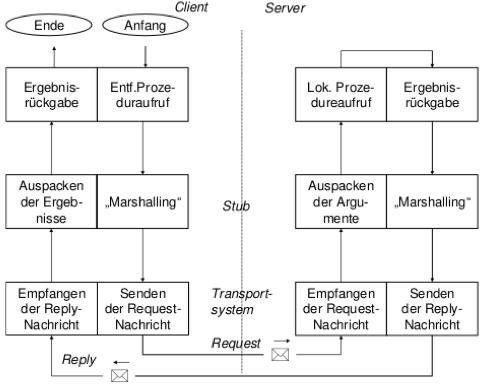
\includegraphics[scale=0.5]{rpc-funktionsweise.png}\\
\end{center}

\subsection{Server / Client Bindung}
\begin{itemize}
	\item Finden eines Servers im Netz
	\item Finden des gewünschten Service auf dem Server im Netz
	\item Sun RPC benutzt die Standard-Unix-Methode für das Finden von Servern im Internet (DNS).
	\item Alle Serverprogramme, Programmversionen und angebotenen Prozeduren werden mit eindeutigen Nummern gekennzeichnet.
	\item Ein Prozess kann eine oder mehrere Prozeduren anbieten.
	\item Der protmapper Prozess (Linux: rpcbind) auf Porst 111 auf jedem Serversystem dient als zentrale, lokale Registratur für verfügbare RPC-Dienste.
\end{itemize}

\subsection{RPC Portmapping Ablauf}
\begin{itemize}
	\item[1.] Der Server erstellt einen Socket und registriert Programmnummer, Versionsnummer und Portnummer beim Portmapper.
	\item[2.] Ein Client kontaktiert den Portmapper und fragt nach einer Programm-, Versions- und Prozedurnummer. Falls lokal bekannt, sendet der Portmapper die Portnummer zurück.
	\item[3./4.] Der Client kann nun die gewünschte Prozedur direkt beim Server aufrufen. 
\end{itemize}
\begin{center}
	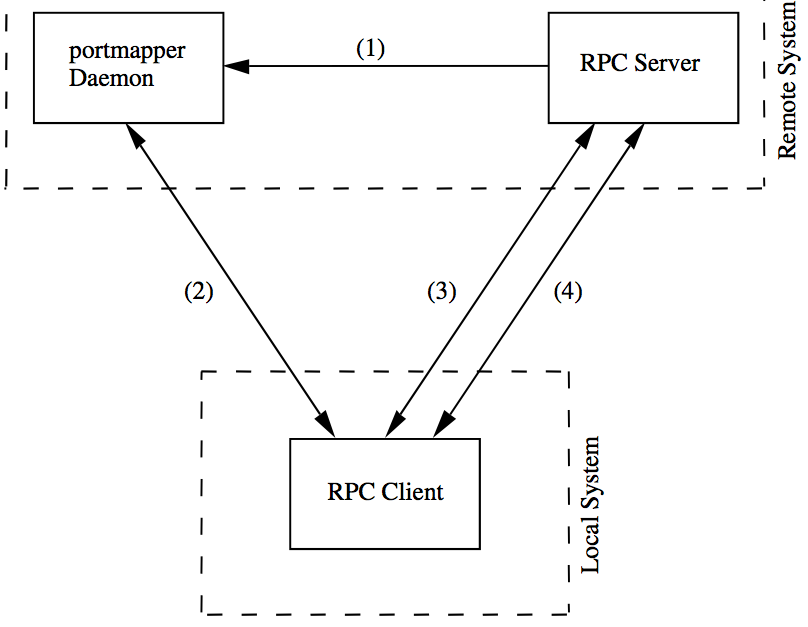
\includegraphics[scale=0.3]{rpc-ablauf.png}\\
\end{center}

\subsection{Auswahl des Transportprotokolls}
\begin{itemize}
	\item RPC ist unabhängig von spezifischen Transportdiensten oder Protokollen. (Sun RPC unterstützt TCP und UDP)
	\item Es werden Abbildungen auf die üblichen Transportprotokolle angeboten.
\end{itemize}

\subsection{Programmierbeispiel}
\begin{center}
	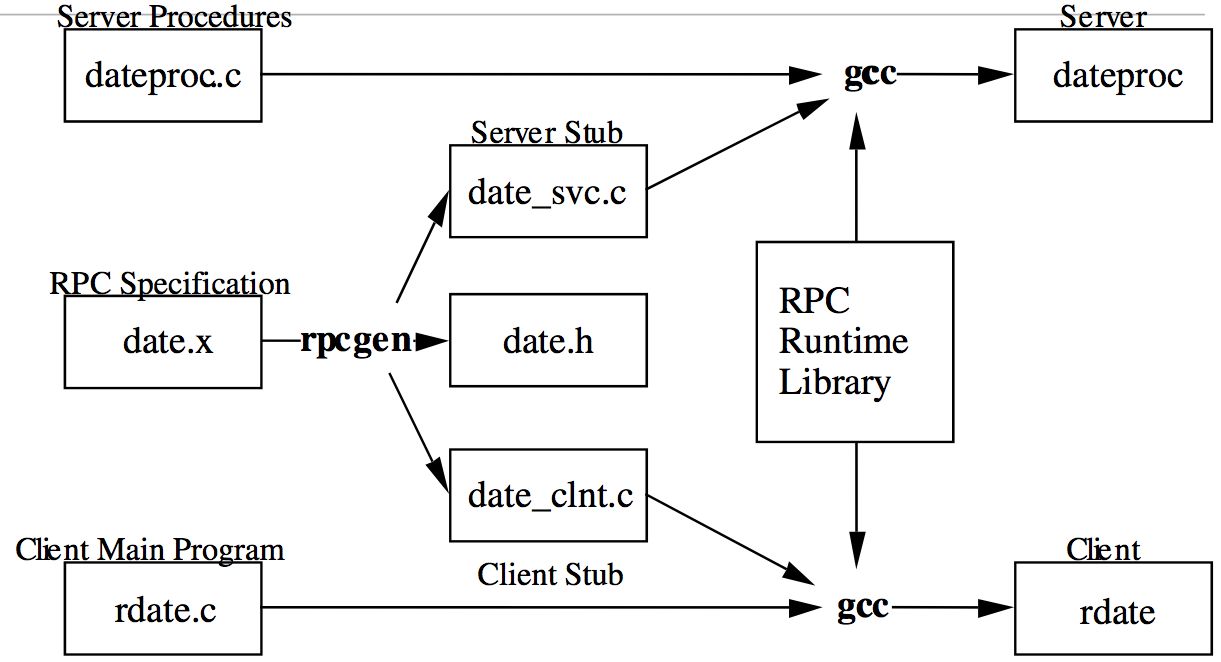
\includegraphics[scale=0.3]{rpc-beispiel.png}\\
\end{center}

\subsection{Ausnahmebehandlung}
\begin{itemize}
	\item Zusätzlich zu lokalen Fehlern können in RPC weitere Fehler auf dem Serversystem und bei der Datenübermittlung durch das Netz auftreten.
	\item Abbruch von bereits übermittelten oder gestarteten Prozeduraufrufen durch den Klienten beim Server.
	\item Terminieren des Klienten bevor der Server den Ablauf der entfernten Prozdedur beendet hat.
	\item Sun RPC verwendet das automatische Neusenden von Anfragen im Fall der Benutzung von UDP, und erkennt verlorene Verbindungen in TCP.
	\item Sun RPC unterstützt keinen separaten Kontrollkanal.
\end{itemize}

\subsection{Aufrufsemantik}
\begin{itemize}
	\item Prozedur wird genau einmal ausgeführt
	\item Prozedur wird höchstens einmal ausgeführt
	\item Prozedur wird mindestens einmal ausgeführt
	\item Jeder Server unterhält einen Cache mit kürzlich erhaltenen Prozeduraufrufen und den zurückgesendeten Resultaten, und sendet das gespeicherte Resultat zurück, wenn ein Duplikat eines PRozeduraufrufs entdeckt wird.
\end{itemize}

\subsection{Benutzung und Beschränkungen}
\begin{itemize}
	\item Die Server sind meist zustandslos:
		\begin{itemize}
			\item alle Operationen sind unabhängig voneinander
			\item Bobustheit gegen Fehler im Klienten, im Server und im Netz
		\end{itemize}
	\item Performance (lokale vs. entfernte Prozeduren)
	\item Service-Strategien (ein Server, ein Server pro Klient, ...)
	\item Verteilungsstrategien (wo im Netz werden Server plaziert.
\end{itemize}
% Inhalt Ende 
\end{document} 